\documentclass[aspectratio=1610,english]{beamer} %If you want to create Polish presentation, replace 'english' with 'polish' and uncomment 3-th line, i.e., '\usepackage{polski}'
\usepackage[utf8]{inputenc}
%\usepackage{polski} %Uncomment for Polish language
\usepackage{babel}
\usepackage{listings} %We want to put listings

\mode<beamer>{ 	%in 'beamer' mode
	\hypersetup{pdfpagemode=FullScreen}		%Enable Full screen mode
	\usetheme[parttitle=rightfooter]{AGH}		%Show part title in right footer
	%\usetheme[nosidebar]{AGH}			%Do not show sidebar on non-title slides
	%\usetheme[nosidebar,margins=1em]{AGH}		%Do not show sidebar on non-title slidesa and set both margins (left / right) to 1em
	%\usetheme[dark]{AGH}                 		%Use dark background
	%\usetheme[dark,parttitle=leftfooter]{AGH}  	%Use dark background and show part title in left footer
}
\mode<handout>{	%in 'handout' mode
	\hypersetup{pdfpagemode=None}		
	\usepackage{pgfpages}
  	\pgfpagesuselayout{4 on 1}[a4paper,border shrink=5mm,landscape]	%show 4 slides on 1 page
  	\usetheme{boxes}
  	\addheadbox{structure}{\quad\insertpart\hfill\insertsection\hfill\insertsubsection\qquad} 	%content of header
 	\addfootbox{structure}{\quad\insertauthor\hfill\insertframenumber\hfill\insertsubtitle\qquad} 	%content of footer
}

\AtBeginPart{ %At begin part: display its name
	\frame{\partpage}
} 

\title{Transfer Learning for Convolutional Neural Networks}
\author{Paweł Kazimierowicz, Kacper Żuk}
\date{}
\institute[AGH]{

}
%%%%%%%%%%% Configuration of the listings package %%%%%%%%%%%%%%%%%%%%%%%%%%
% Source: https://en.wikibooks.org/wiki/LaTeX/Source_Code_Listings#Using_the_listings_package
%%%%%%%%%%%%%%%%%%%%%%%%%%%%%%%%%%%%%%%%%%%%%%%%%%%%%%%%%%%%%%%%%%%%%%%%%%%%
\lstset{ %
  backgroundcolor=\color{white},   % choose the background color
  basicstyle=\footnotesize,        % the size of the fonts that are used for the code
  breakatwhitespace=false,         % sets if automatic breaks should only happen at whitespace
  breaklines=true,                 % sets automatic line breaking
  captionpos=b,                    % sets the caption-position to bottom
  commentstyle=\color{green},      % comment style
  deletekeywords={...},            % if you want to delete keywords from the given language
  escapeinside={\%*}{*)},          % if you want to add LaTeX within your code
  extendedchars=true,              % lets you use non-ASCII characters; for 8-bits encodings only, does not work with UTF-8
  frame=single,	                   % adds a frame around the code
  keepspaces=true,                 % keeps spaces in text, useful for keeping indentation of code (possibly needs columns=flexible)
  keywordstyle=\color{blue},       % keyword style
  morekeywords={*,...},            % if you want to add more keywords to the set
  numbers=left,                    % where to put the line-numbers; possible values are (none, left, right)
  numbersep=5pt,                   % how far the line-numbers are from the code
  numberstyle=\tiny\color{gray},   % the style that is used for the line-numbers
  rulecolor=\color{black},         % if not set, the frame-color may be changed on line-breaks within not-black text (e.g. comments (green here))
  showspaces=false,                % show spaces everywhere adding particular underscores; it overrides 'showstringspaces'
  showstringspaces=false,          % underline spaces within strings only
  showtabs=false,                  % show tabs within strings adding particular underscores
  stepnumber=2,                    % the step between two line-numbers. If it's 1, each line will be numbered
  stringstyle=\color{cyan},        % string literal style
  tabsize=2,	                   % sets default tabsize to 2 spaces
  title=\lstname,                  % show the filename of files included with \lstinputlisting; also try caption instead of title
                                   % needed if you want to use UTF-8 Polish chars
  literate={ą}{{\k{a}}}1
           {Ą}{{\k{A}}}1
           {ę}{{\k{e}}}1
           {Ę}{{\k{E}}}1
           {ó}{{\'o}}1
           {Ó}{{\'O}}1
           {ś}{{\'s}}1
           {Ś}{{\'S}}1
           {ł}{{\l{}}}1
           {Ł}{{\L{}}}1
           {ż}{{\.z}}1
           {Ż}{{\.Z}}1
           {ź}{{\'z}}1
           {Ź}{{\'Z}}1
           {ć}{{\'c}}1
           {Ć}{{\'C}}1
           {ń}{{\'n}}1
           {Ń}{{\'N}}1
}
%%%%%%%%%%%%%%%%%
\begin{document}
  	\maketitle
	\part{Why Transfer Learning is fun and profit?}
	\section{Introduction}
		\begin{frame}{What will be talking about?}
			Transfer learning (Inductive transfer) for Convolutional Neural Networks (ConvNets). 
			\newline
			\newline
			Process where structure or knowledge from a learning problem is used to enhance learning on a related problem\footnote{West, Jeremy; Ventura, Dan; Warnick, Sean (2007), "A Theoretical Foundation for Inductive Transfer", \url{http://cpms.byu.edu/springresearch/abstract-entry?id=861}}. 
			\newline
			\newline
			Example: \newline
			Take an image classification model that is capable to correctly label common objects (a dog, a tree or an airplane)
			\newline 
			Retrain it to label types of yoghurt on a production lane.
		\end{frame}
	
	\section{Steps needed to be designed for image classification model:}
	\begin{frame}{First of all - why do we need Transfer Learning?}
		There is a lot of to be designed to build an image classification model:
		\begin{itemize}
			\item first layer:
			\begin{itemize}
				\item data preprocessing,
				\item feature extraction,
			\end{itemize}

		\item middle layers:
			\begin{itemize}
				\item what shall be in the middle layers
				\item btw, what kind of a network shall it be?
			\end{itemize}
		
		\item the last layer:
			\begin{itemize}
				\item actual classification and labels.
			\end{itemize}
		\end{itemize}
	 \end{frame}
 
 	\begin{frame}{Sounds easy, but in reality it looks something like this...}
 	\centering
	 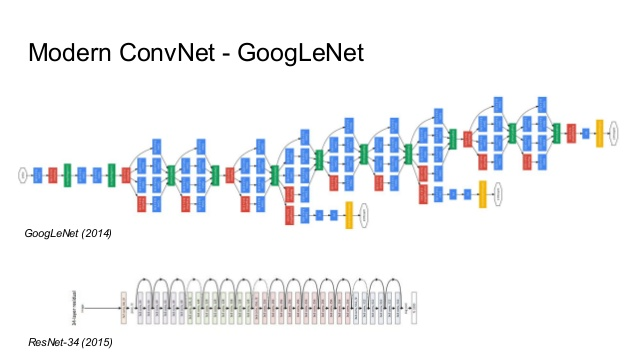
\includegraphics[scale=0.6]{images/design}
	\end{frame}
 
	\begin{frame}{But there is a problem...}
		We usually don't really know what is the best solution to our specific case scenario.
		\newline
		\newline
		Usual methods consist of trial and error, blind luck, and intuition.
	
	 \end{frame}
 
 	\section{But there is a lot of well designed models}
	\begin{frame}{Big minds have done it better (probably)}
	Huge research centers and companies have the knowledge and resources to design and train good models:
		 \begin{itemize}
		 	\item they have huge amounts of data (ImageNet has around 14 million of labeled images!)
		 	\item these models have been already trained (training on GPU can take weeks)
		 \end{itemize}
	\end{frame}

	\begin{frame}{Labeling the images takes time and patience...}
		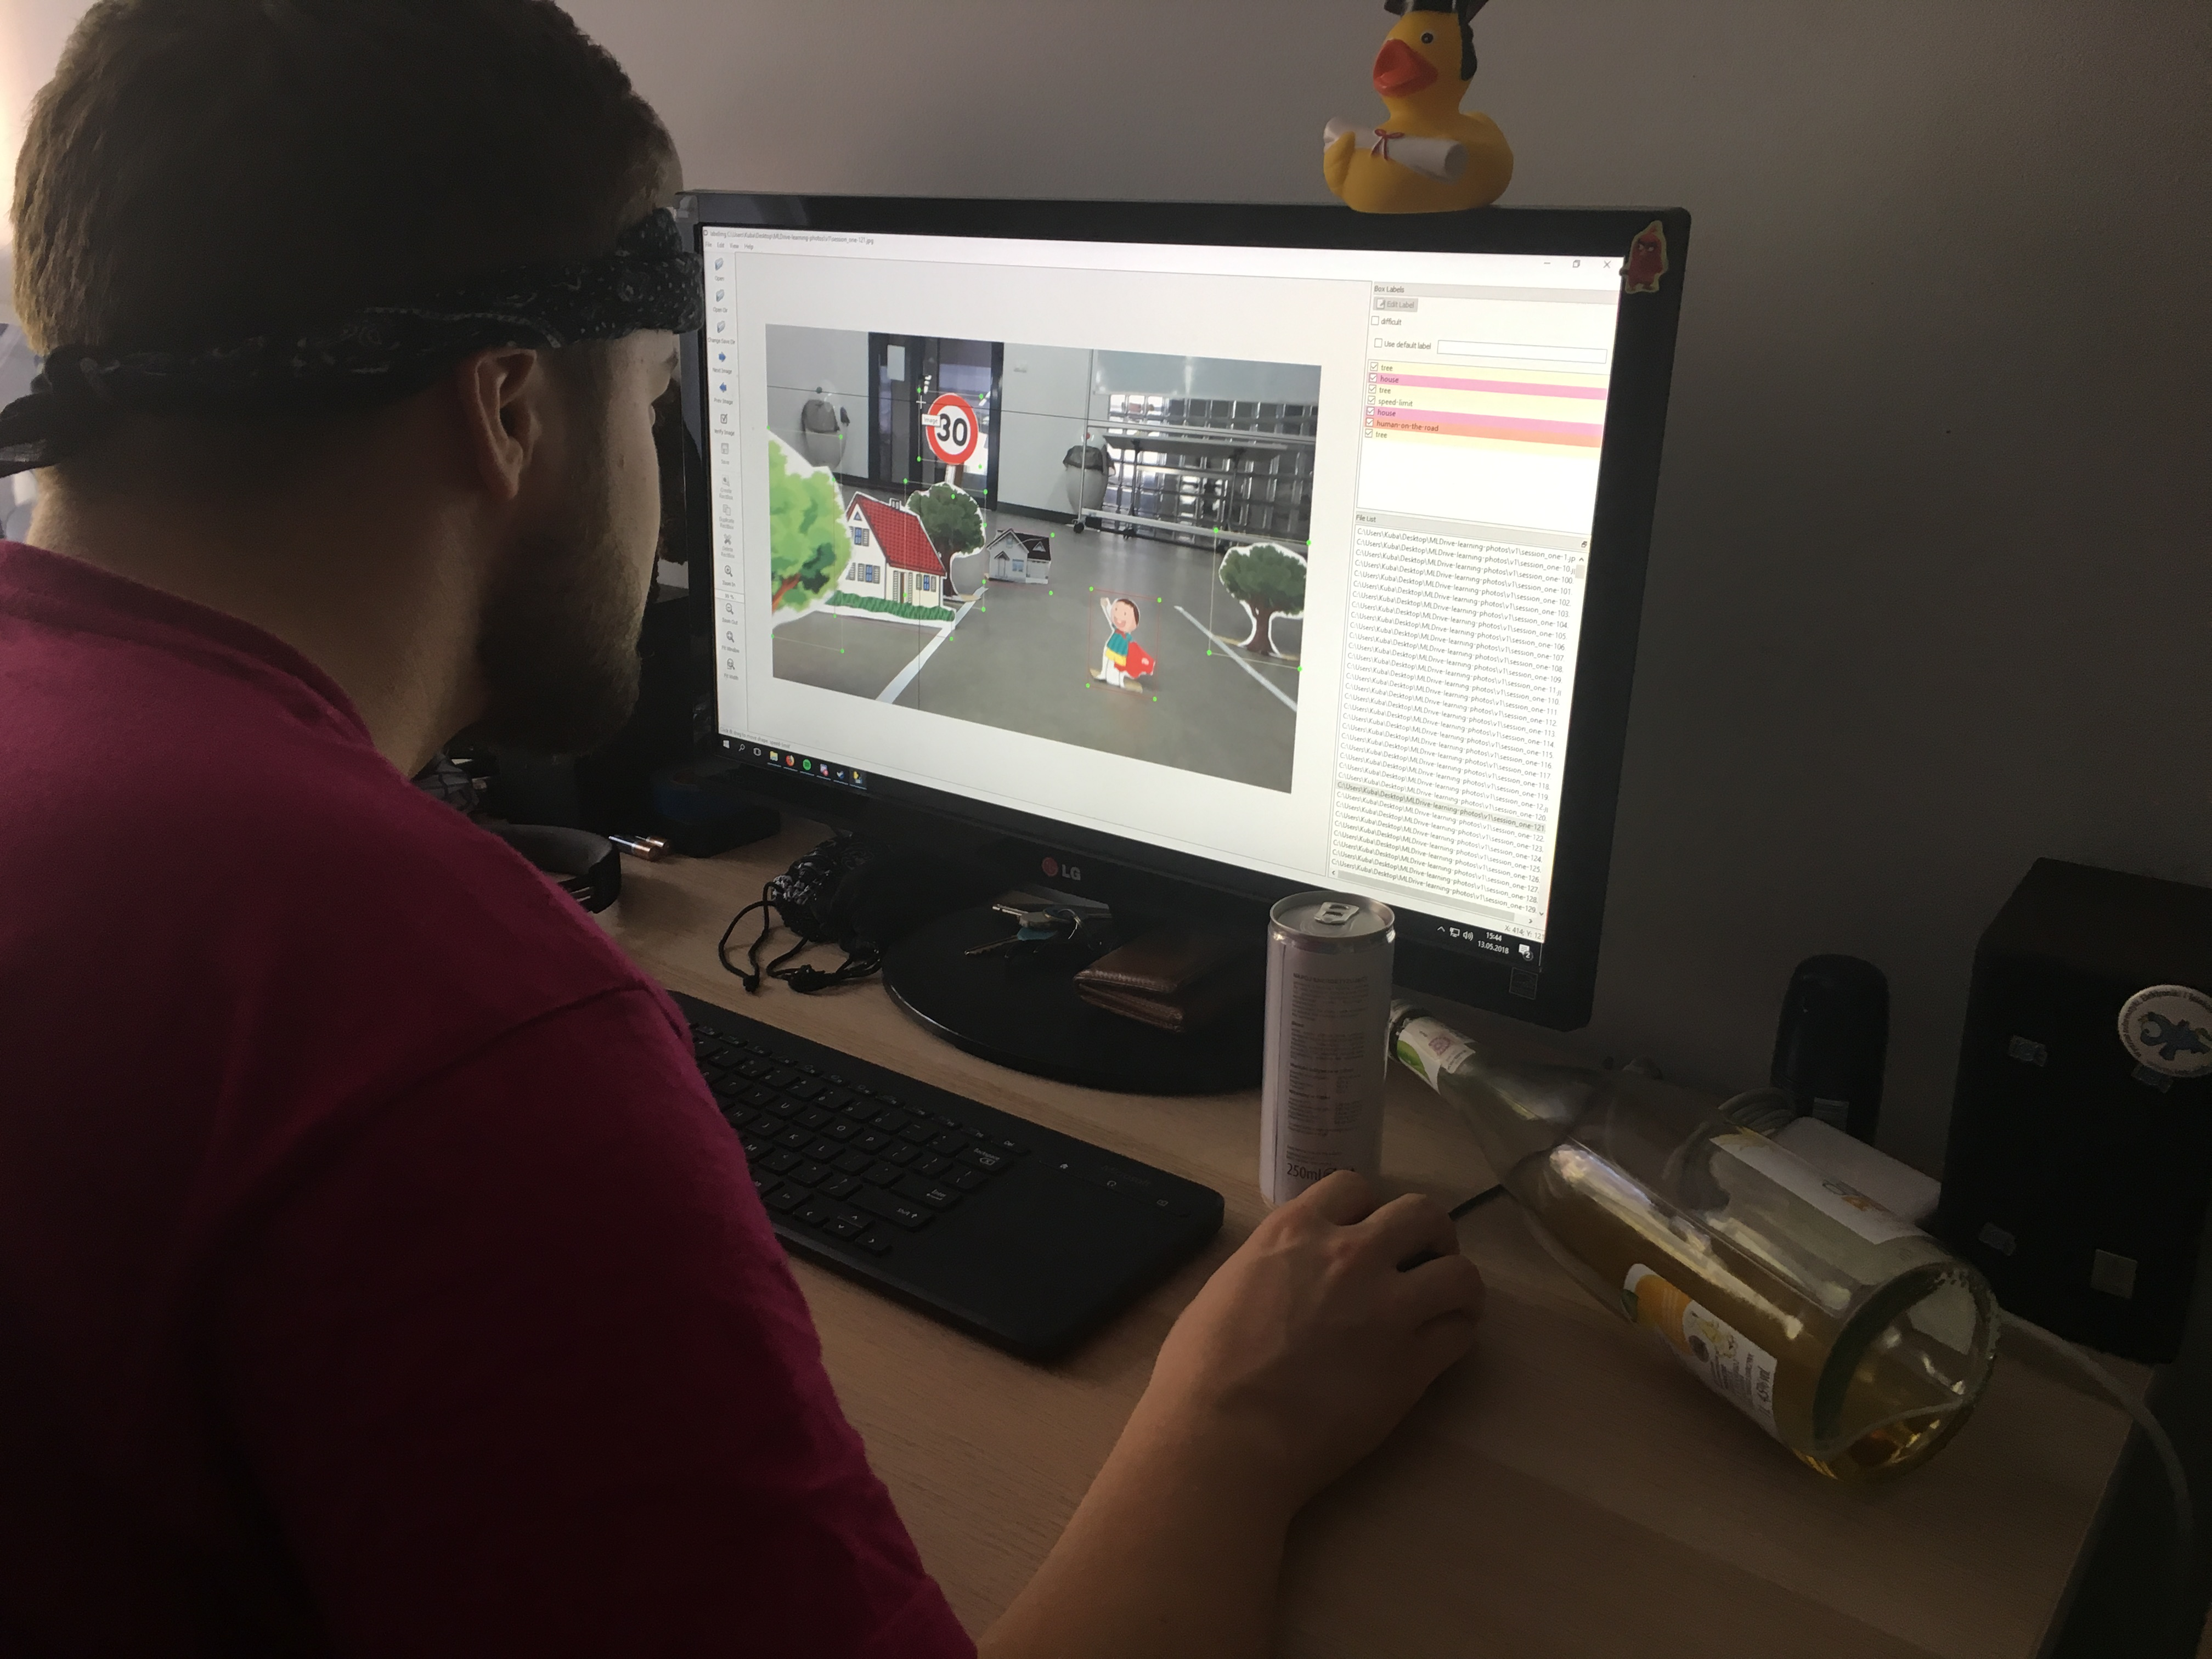
\includegraphics[scale=0.1]{images/kuba}
	\end{frame}

 	\begin{frame}{Can we just take a pretrained model and use it?}
 		Of course we can, but:
		 \begin{itemize}
		 	\item it will not exactly work,
		 	\item there is difference between butterflies, airplanes and printed circuit boards.
		 \end{itemize}
	\end{frame}

\section{So, what is this tranfer learning for real?}
 	\begin{frame}{Can we train the defined model on our dataset?}
 	We can take some shortcuts:
		\begin{itemize}
			\item let's say that we have a huge amount of labeled data - that's cool,
			\item we're no researchers - we can take already designed neural network scheme,
			\item after training it on our dataset - we might expect good results.
		\end{itemize}
	\end{frame}
 
 	\begin{frame}{But what if I don't have a huge dataset?}
 		If we have a significantly smaller dataset, we could try:
 		\begin{itemize}
		 	\item take the weights from the model as it is already trained on some huge, generic dataset,
		 	\item retrain it from this point on our dataset - possibly freezing first and maybe even middle layers,
		 	\item depending on how similar our problem is to the original one - that good results.
		 \end{itemize}
	\end{frame}

\section{But first, let's talk a bit about theory...}
  	\begin{frame}{How does transfer learning work?}
			 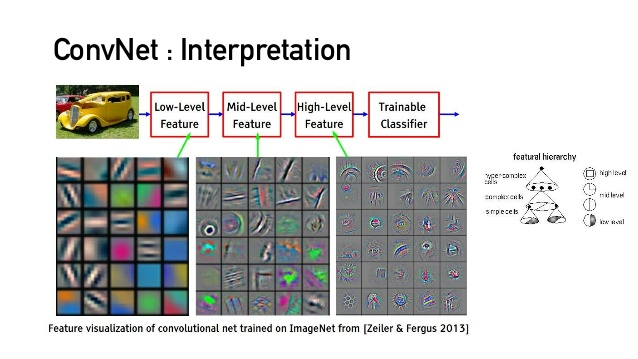
\includegraphics[scale=0.6]{images/interpr}
	 \end{frame}
  	\begin{frame}{Let's sum this up!}
		We have three approaches possible to transfer learning:
		 \begin{itemize}
		 	\item take the model as it is - and use it,
		 	\item take the model structure and train it on our (huge) dataset,
		 	\item take the model and it's weights and train it on our smaller dataset.
		 \end{itemize}
	\end{frame}
 \section{Once again - will this really work?}
  	\begin{frame}{Examples}
		For our examples, we've taken Google's MobileNet (\url{https://arxiv.org/abs/1704.04861}) model, using reference TensorFlow implementation. We've also downloaded weights trained on the COCO dataset (\url{http://cocodataset.org/\#home}).\newline
		We've only done 1000 steps of training with learning rate equal to 0.003.\newline
		Our dataset consisted of only 360 labeled photos.
	\end{frame}
	\begin{frame}{Examples - COCO}
		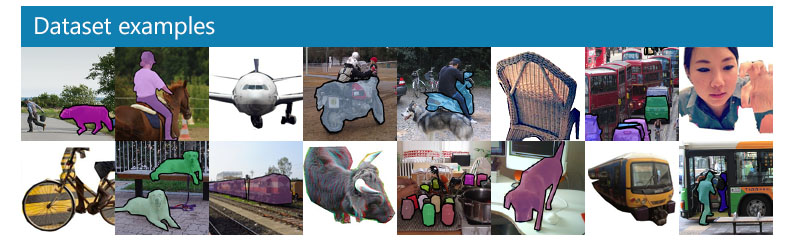
\includegraphics[scale=0.5]{images/coco-examples}
	\end{frame}

  	\begin{frame}{Examples - first example}
		First example used weights trained on the COCO dataset and used this as a base for training on our dataset.
	\end{frame}
  	\begin{frame}{Examples}
		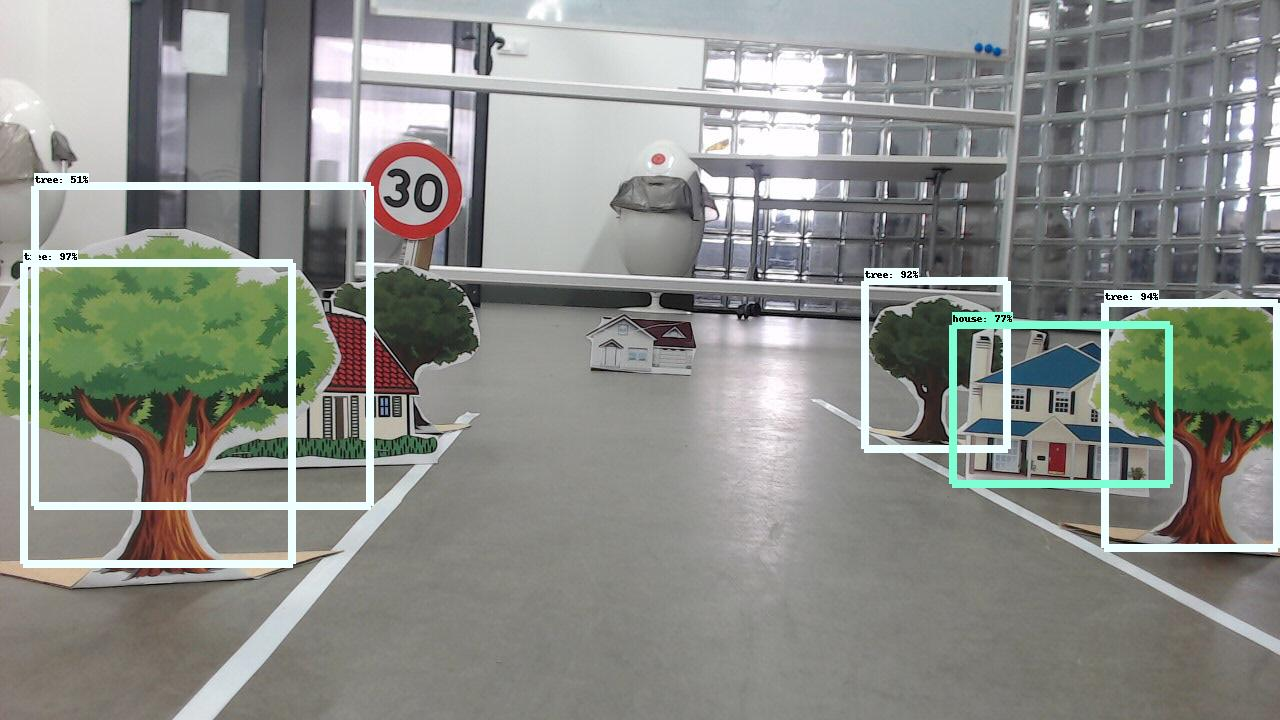
\includegraphics[scale=0.3]{examples/comparison_1000_step/session_one-6.jpg}
	\end{frame}
  	\begin{frame}{Examples}
		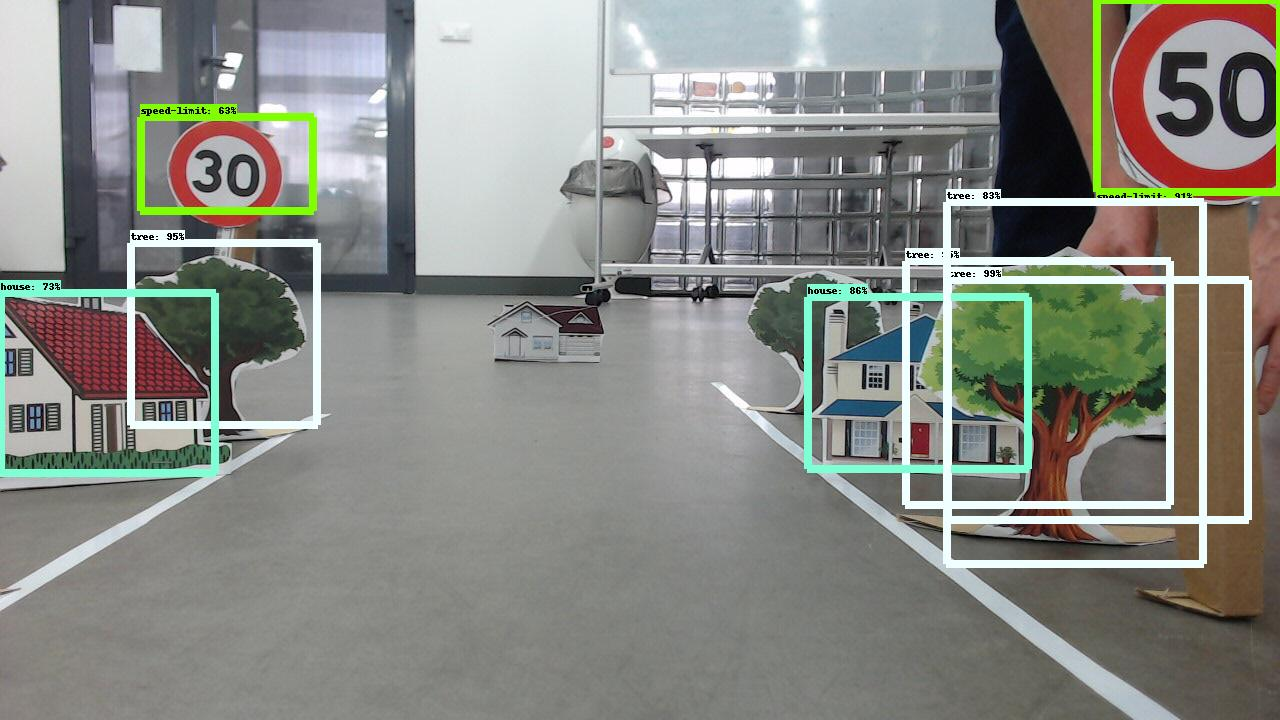
\includegraphics[scale=0.3]{examples/comparison_1000_step/session_one-10.jpg}
	\end{frame}
	
  	\begin{frame}{Examples - second example}
		Second example used the MobileNet model with weights trained on COCO dataset without additional training on our dataset.
	\end{frame}
  	\begin{frame}{Examples}
		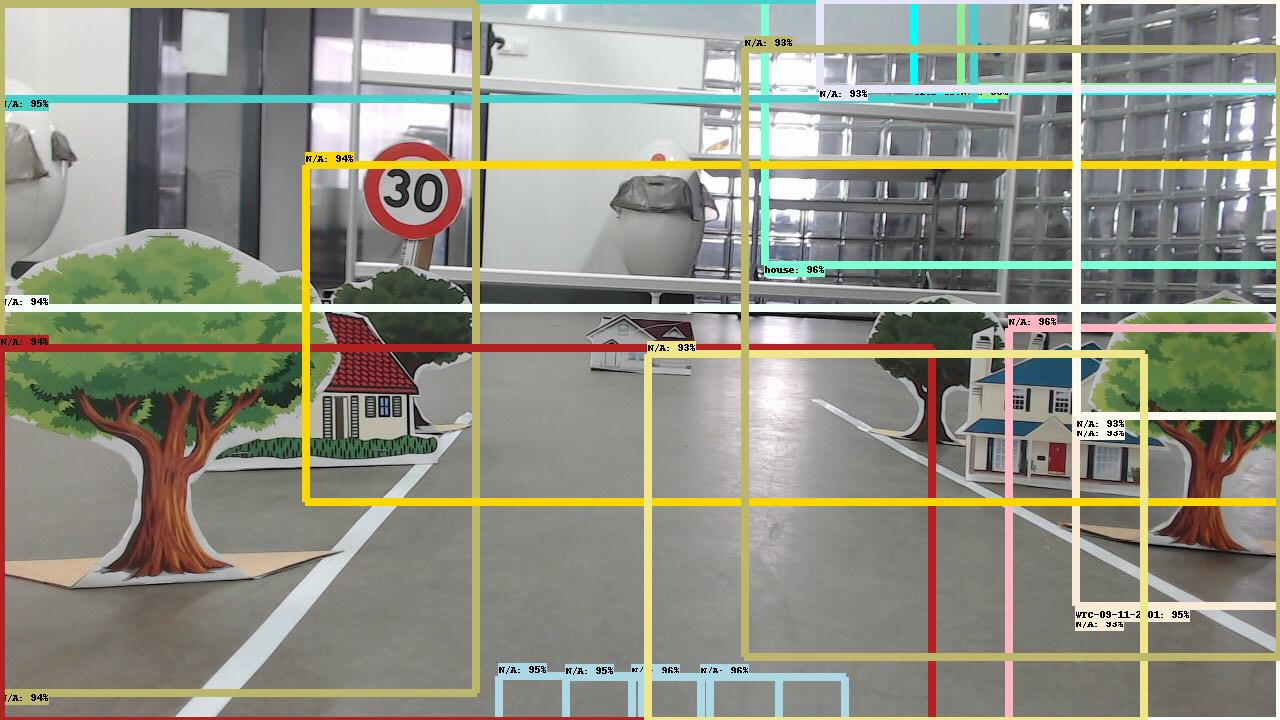
\includegraphics[scale=0.3]{examples/no_retraining_of_stock_model/session_one-6.jpg}
	\end{frame}
  	\begin{frame}{Examples}
		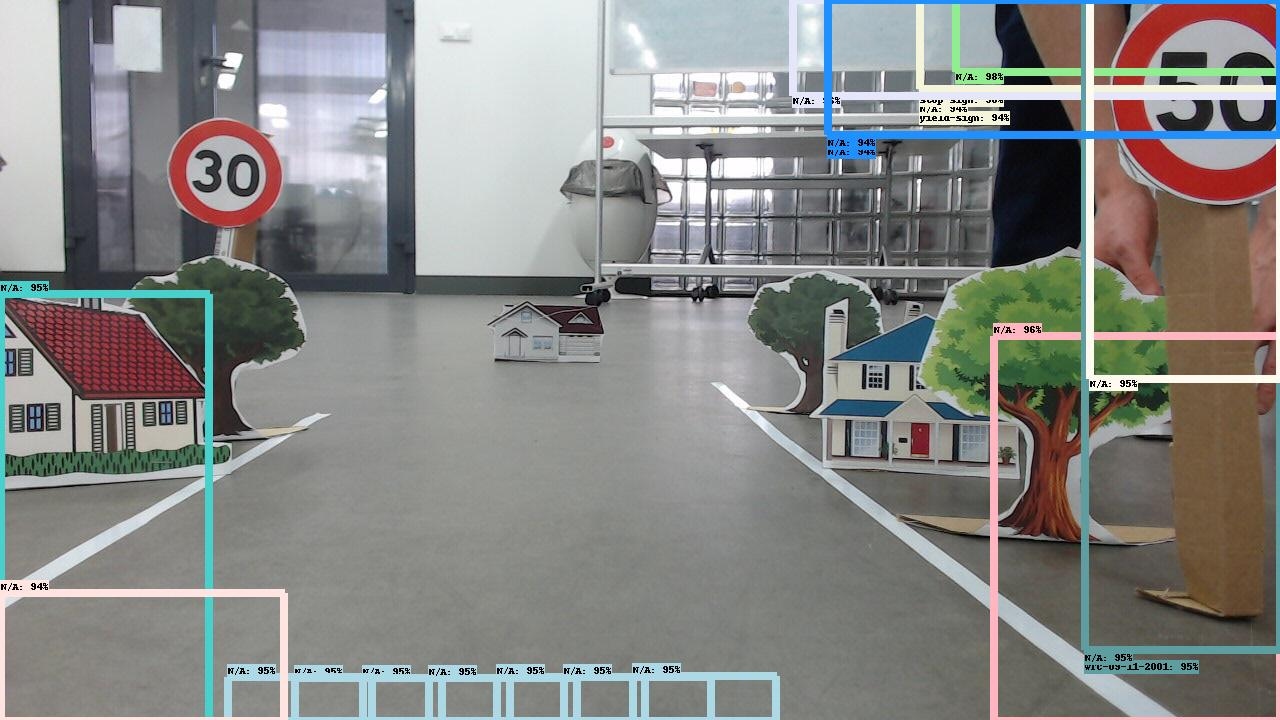
\includegraphics[scale=0.3]{examples/no_retraining_of_stock_model/session_one-10.jpg}
	\end{frame}
	
	
  	\begin{frame}{Examples - third example}
		Third example used the MobileNet model with random initial weights.
	\end{frame}
  	\begin{frame}{Examples}
		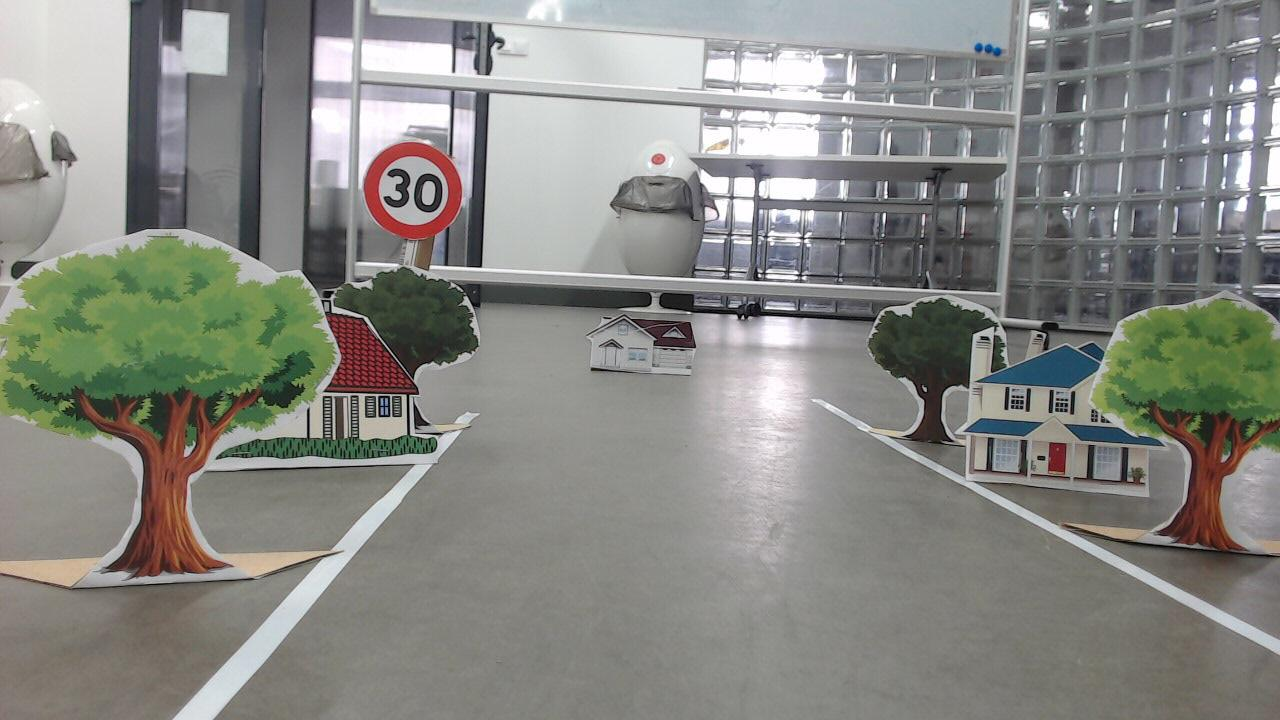
\includegraphics[scale=0.3]{examples/no_fine_tune_checkpoint_1000_step/session_one-6.jpg}
	\end{frame}
  	\begin{frame}{Examples}
		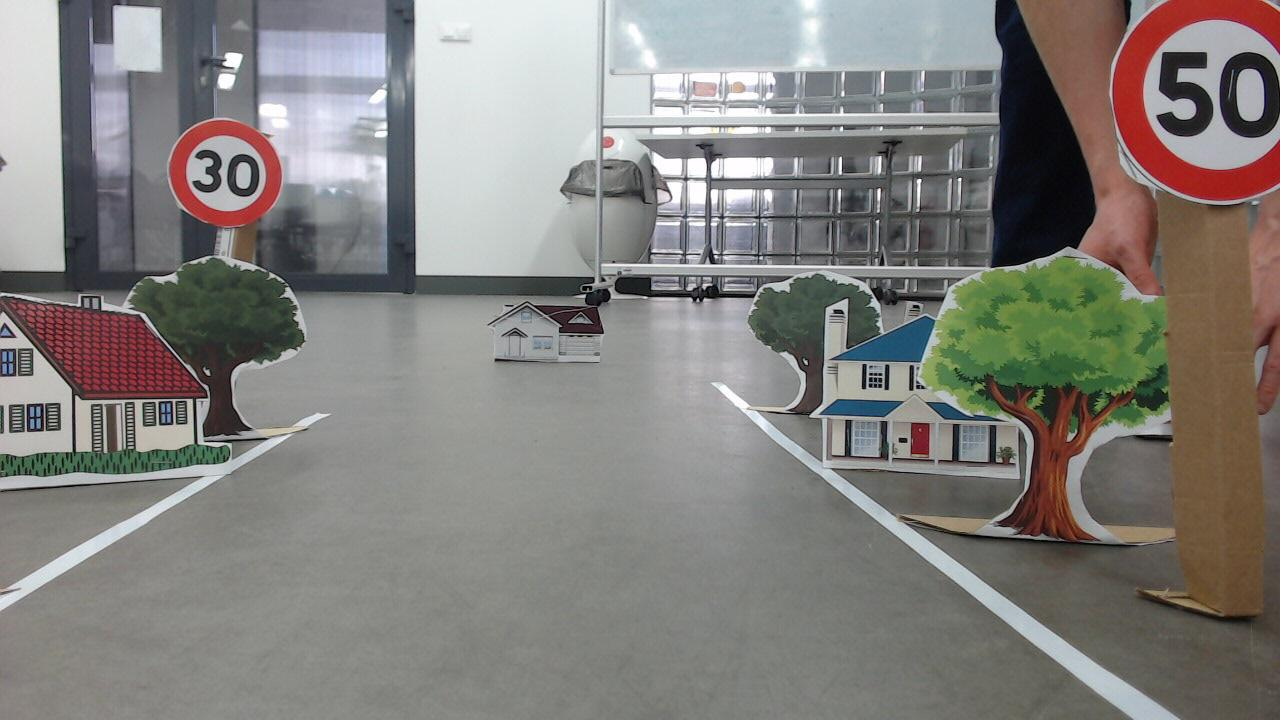
\includegraphics[scale=0.3]{examples/no_fine_tune_checkpoint_1000_step/session_one-10.jpg}
	\end{frame}
	
  	
  	\section{Talk is cheap. Show me the code!}
	\begin{frame}{Examples}
	Example time!
	\end{frame}
	
	
\part{Time for you to build your own \textit{teslas}!}
	\begin{frame}{How to get started easily}
	Follow the instructions here:
	\url{https://github.com/pkazimierowicz/AI_TransferLearning_exercise}
	\end{frame}

\end{document}

